\section{Tổng quan dữ liệu đầu vào}

Chương này trình bày chi tiết kết quả phân tích khám phá dữ liệu (EDA) trên toàn bộ tập mẫu đã thu thập. Mục tiêu chính là nắm bắt phân bố dữ liệu, khảo sát các đặc trưng thống kê cơ bản, và từ đó đề xuất phương án tiền xử lý phù hợp cho cả văn bản và hình ảnh trước khi đưa vào huấn luyện mô hình.

\subsection{Phân tích đặc trưng dữ liệu văn bản}

Khía cạnh văn bản của tập dữ liệu chứa 25.292 bình luận phản hồi từ người tiêu dùng thương mại điện tử, được gán nhãn ở hai cấp độ: nhãn cảm xúc (tích cực, tiêu cực, trung lập) và nhãn bình luận rác (spam). Quá trình đánh giá tập trung vào phân bố dữ liệu và cấu trúc độ dài của từng nhận xét nhằm hiểu rõ hành vi ngôn ngữ của người dùng.

\subsubsection{Chiến lược tiền xử lý văn bản}

Để giải quyết đặc tính nhiễu loạn và thiếu chuẩn mực của các bình luận thương mại điện tử, nhóm nghiên cứu đã thiết lập một pipeline tiền xử lý văn bản chuyên biệt. Thay vì áp dụng tuần tự các bộ lọc cơ bản, quá trình này tích hợp các bước tối ưu hóa sau:
\begin{itemize}[labelsep=10pt, leftmargin=2cm]
    \item \textbf{Làm sạch nhiễu định dạng:} Loại bỏ các đường dẫn URL, thẻ HTML, số điện thoại, email và các ký tự đặc biệt không mang giá trị ngữ nghĩa.
    \item \textbf{Chuẩn hóa teencode và biểu tượng emoji:} Sử dụng từ điển đối chiếu để ánh xạ các từ viết tắt và các biểu tượng cảm xúc mang tín hiệu mạnh (như icon mặt cười, mặt giận) về dạng chữ tiếng Việt chuẩn. Các emoji không xác định sẽ được loại bỏ hoàn toàn.
    \item \textbf{Xử lý ký tự lặp và tách từ:} Nén các chuỗi ký tự lặp kéo dài (ví dụ ``quáaaaa'') về dạng nguyên bản. Sau đó, văn bản được tiến hành tách từ ghép tiếng Việt (sử dụng thư viện \texttt{underthesea}) nhằm bảo toàn ý nghĩa của các từ đa âm tiết trước khi chuyển sang không gian vector hóa.
\end{itemize}

\subsubsection{Phân bố nhãn cảm xúc và nhận diện bình luận rác}

Việc thống kê số lượng mẫu theo từng nhãn giúp nhóm nhận diện tình trạng mất cân bằng dữ liệu, từ đó có hướng điều chỉnh trọng số hoặc trích mẫu phù hợp khi huấn luyện.

\begin{figure}[H]
    \centering
    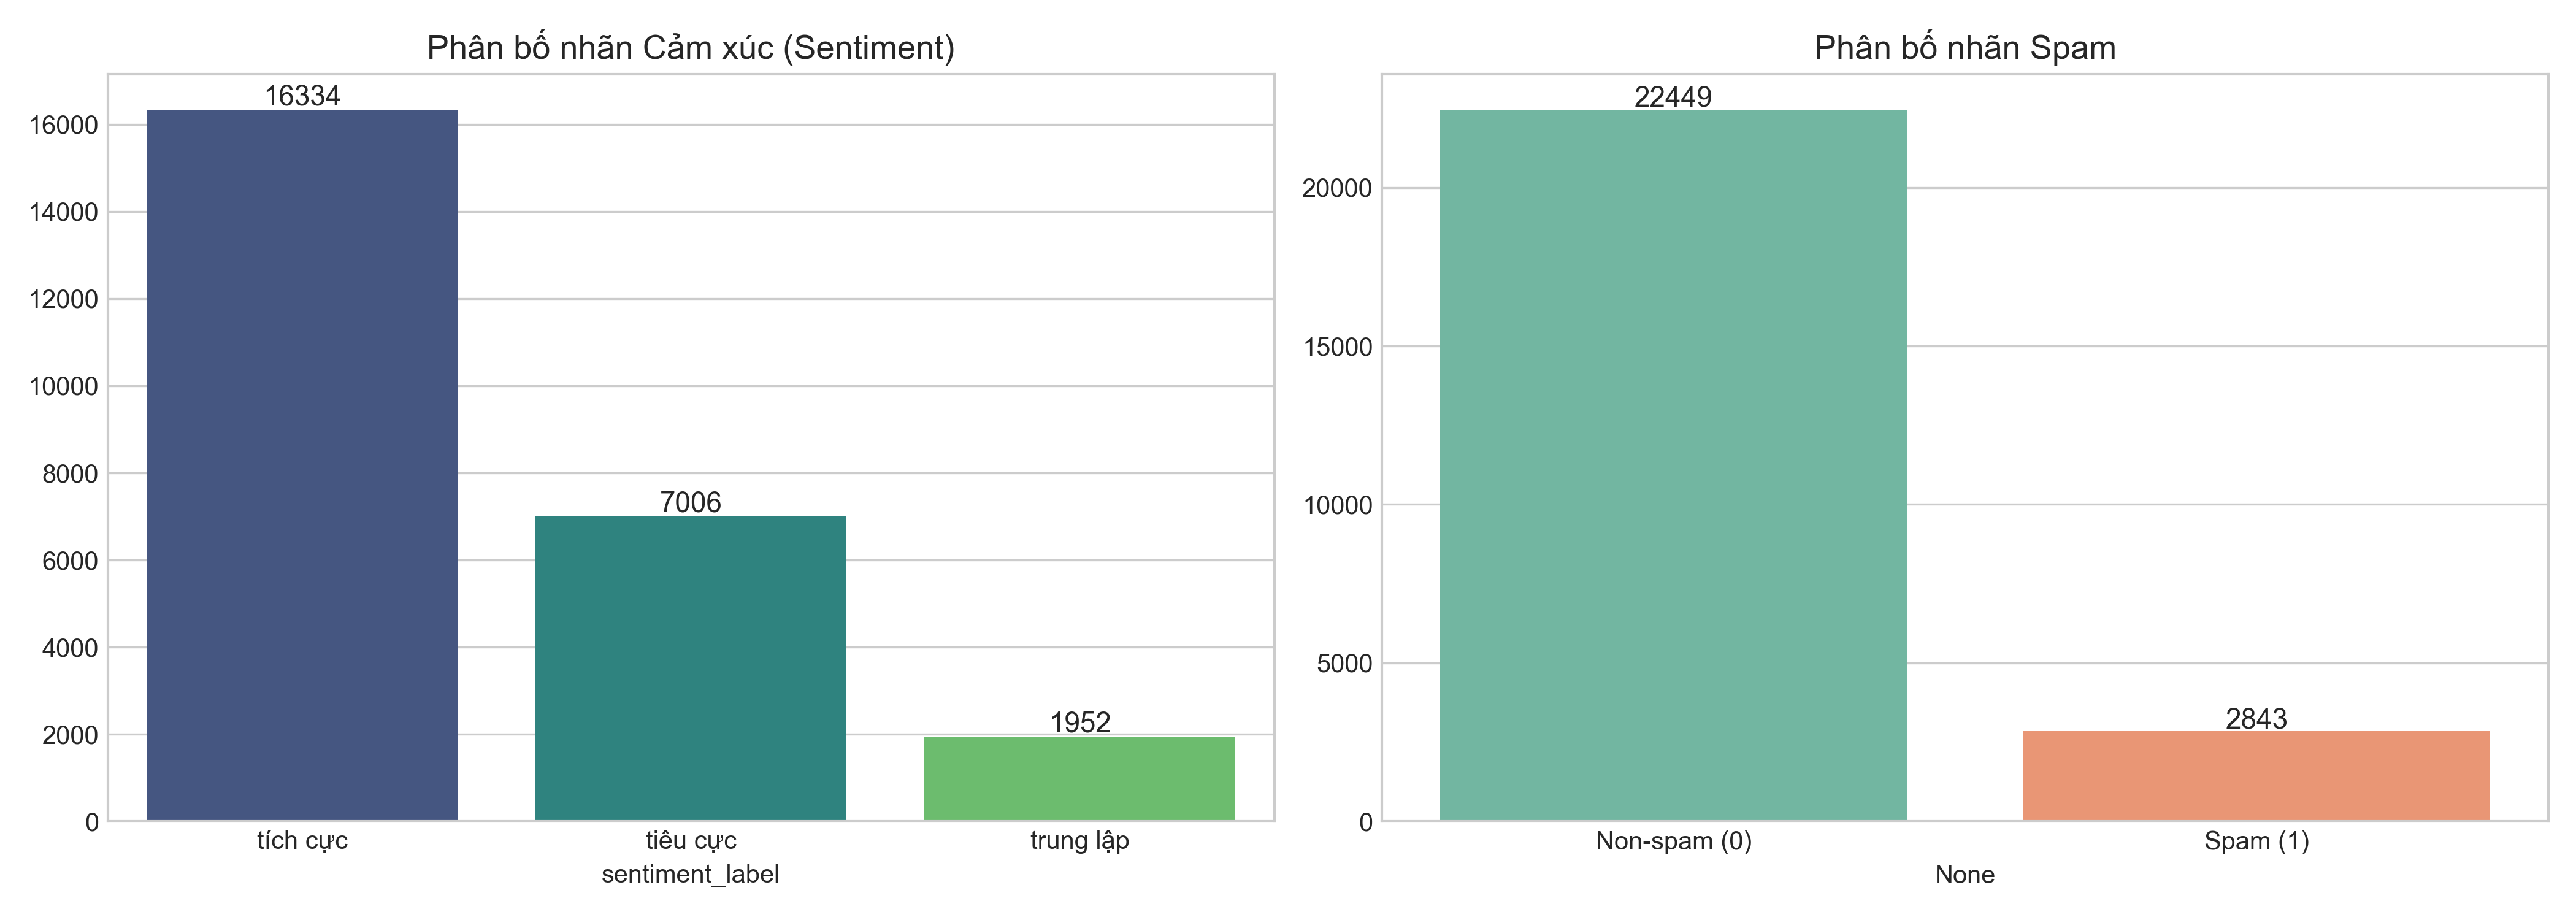
\includegraphics[width=\textwidth]{graphics/text_label_distributions.png}
    \caption[Phân bố nhãn cảm xúc và bình luận rác]{%
      Phân bố nhãn cảm xúc và bình luận rác.\\
      \textit{Ghi chú: Biểu đồ trực quan hóa số lượng mẫu phân theo từng hạng mục nhãn trên tập dữ liệu văn bản.}%
    }
    \label{fig:text_label_distributions}
\end{figure}

Dựa trên Hình~\ref{fig:text_label_distributions}, tập dữ liệu thể hiện sự mất cân bằng rất đặc trưng ở khía cạnh cảm xúc. Cụ thể, nhóm đánh giá tích cực chiếm tỷ trọng áp đảo với 16.334 mẫu (chiếm khoảng 64,6\% tổng tập dữ liệu), phản ánh khuynh hướng chung của người dùng thương mại điện tử thường để lại đánh giá tốt khi giao dịch hoàn tất thành công. Nhóm đánh giá tiêu cực ghi nhận 7.006 mẫu (khoảng 27,7\%), đóng vai trò cung cấp tín hiệu quan trọng về các khiếm khuyết sản phẩm hoặc dịch vụ. Nhóm trung lập là lớp thiểu số hiếm gặp nhất với chỉ 1.952 mẫu (khoảng 7,7\%). Sự chênh lệch tỷ lệ (roughly 8:3:1) này đòi hỏi hệ thống mô hình hóa phải áp dụng các chiến lược phạt lỗi có trọng số hoặc phương pháp trích mẫu phân tầng để duy trì khả năng nhận diện chính xác các lớp thiểu số, tránh việc mô hình bị bias về lớp tích cực.

Bên cạnh đó, phân bố nhãn bình luận rác cũng cho thấy sự lấn lướt của nhóm dữ liệu hợp lệ so với dữ liệu rác. Dù chiếm tỷ lệ nhỏ, nhóm bình luận rác chứa các mẫu nhiễu dạng mẫu câu lặp lại vô nghĩa (như chép phạt, copy-paste) nhằm nhận xu thưởng, có khả năng làm giảm độ nhạy của mô hình ngôn ngữ nếu không được thanh lọc tốt.

\subsubsection{Cấu trúc độ dài văn bản theo nhóm cảm xúc}

Để hiểu rõ hơn về hành vi biểu đạt của người dùng, chiều dài của văn bản tính theo số lượng từ được khảo sát chi tiết. Thống kê chỉ ra rằng nhóm tích cực có trung bình 21,76 từ, tiêu cực là 17,65 từ và trung lập là 15,48 từ.

\begin{figure}[H]
    \centering
    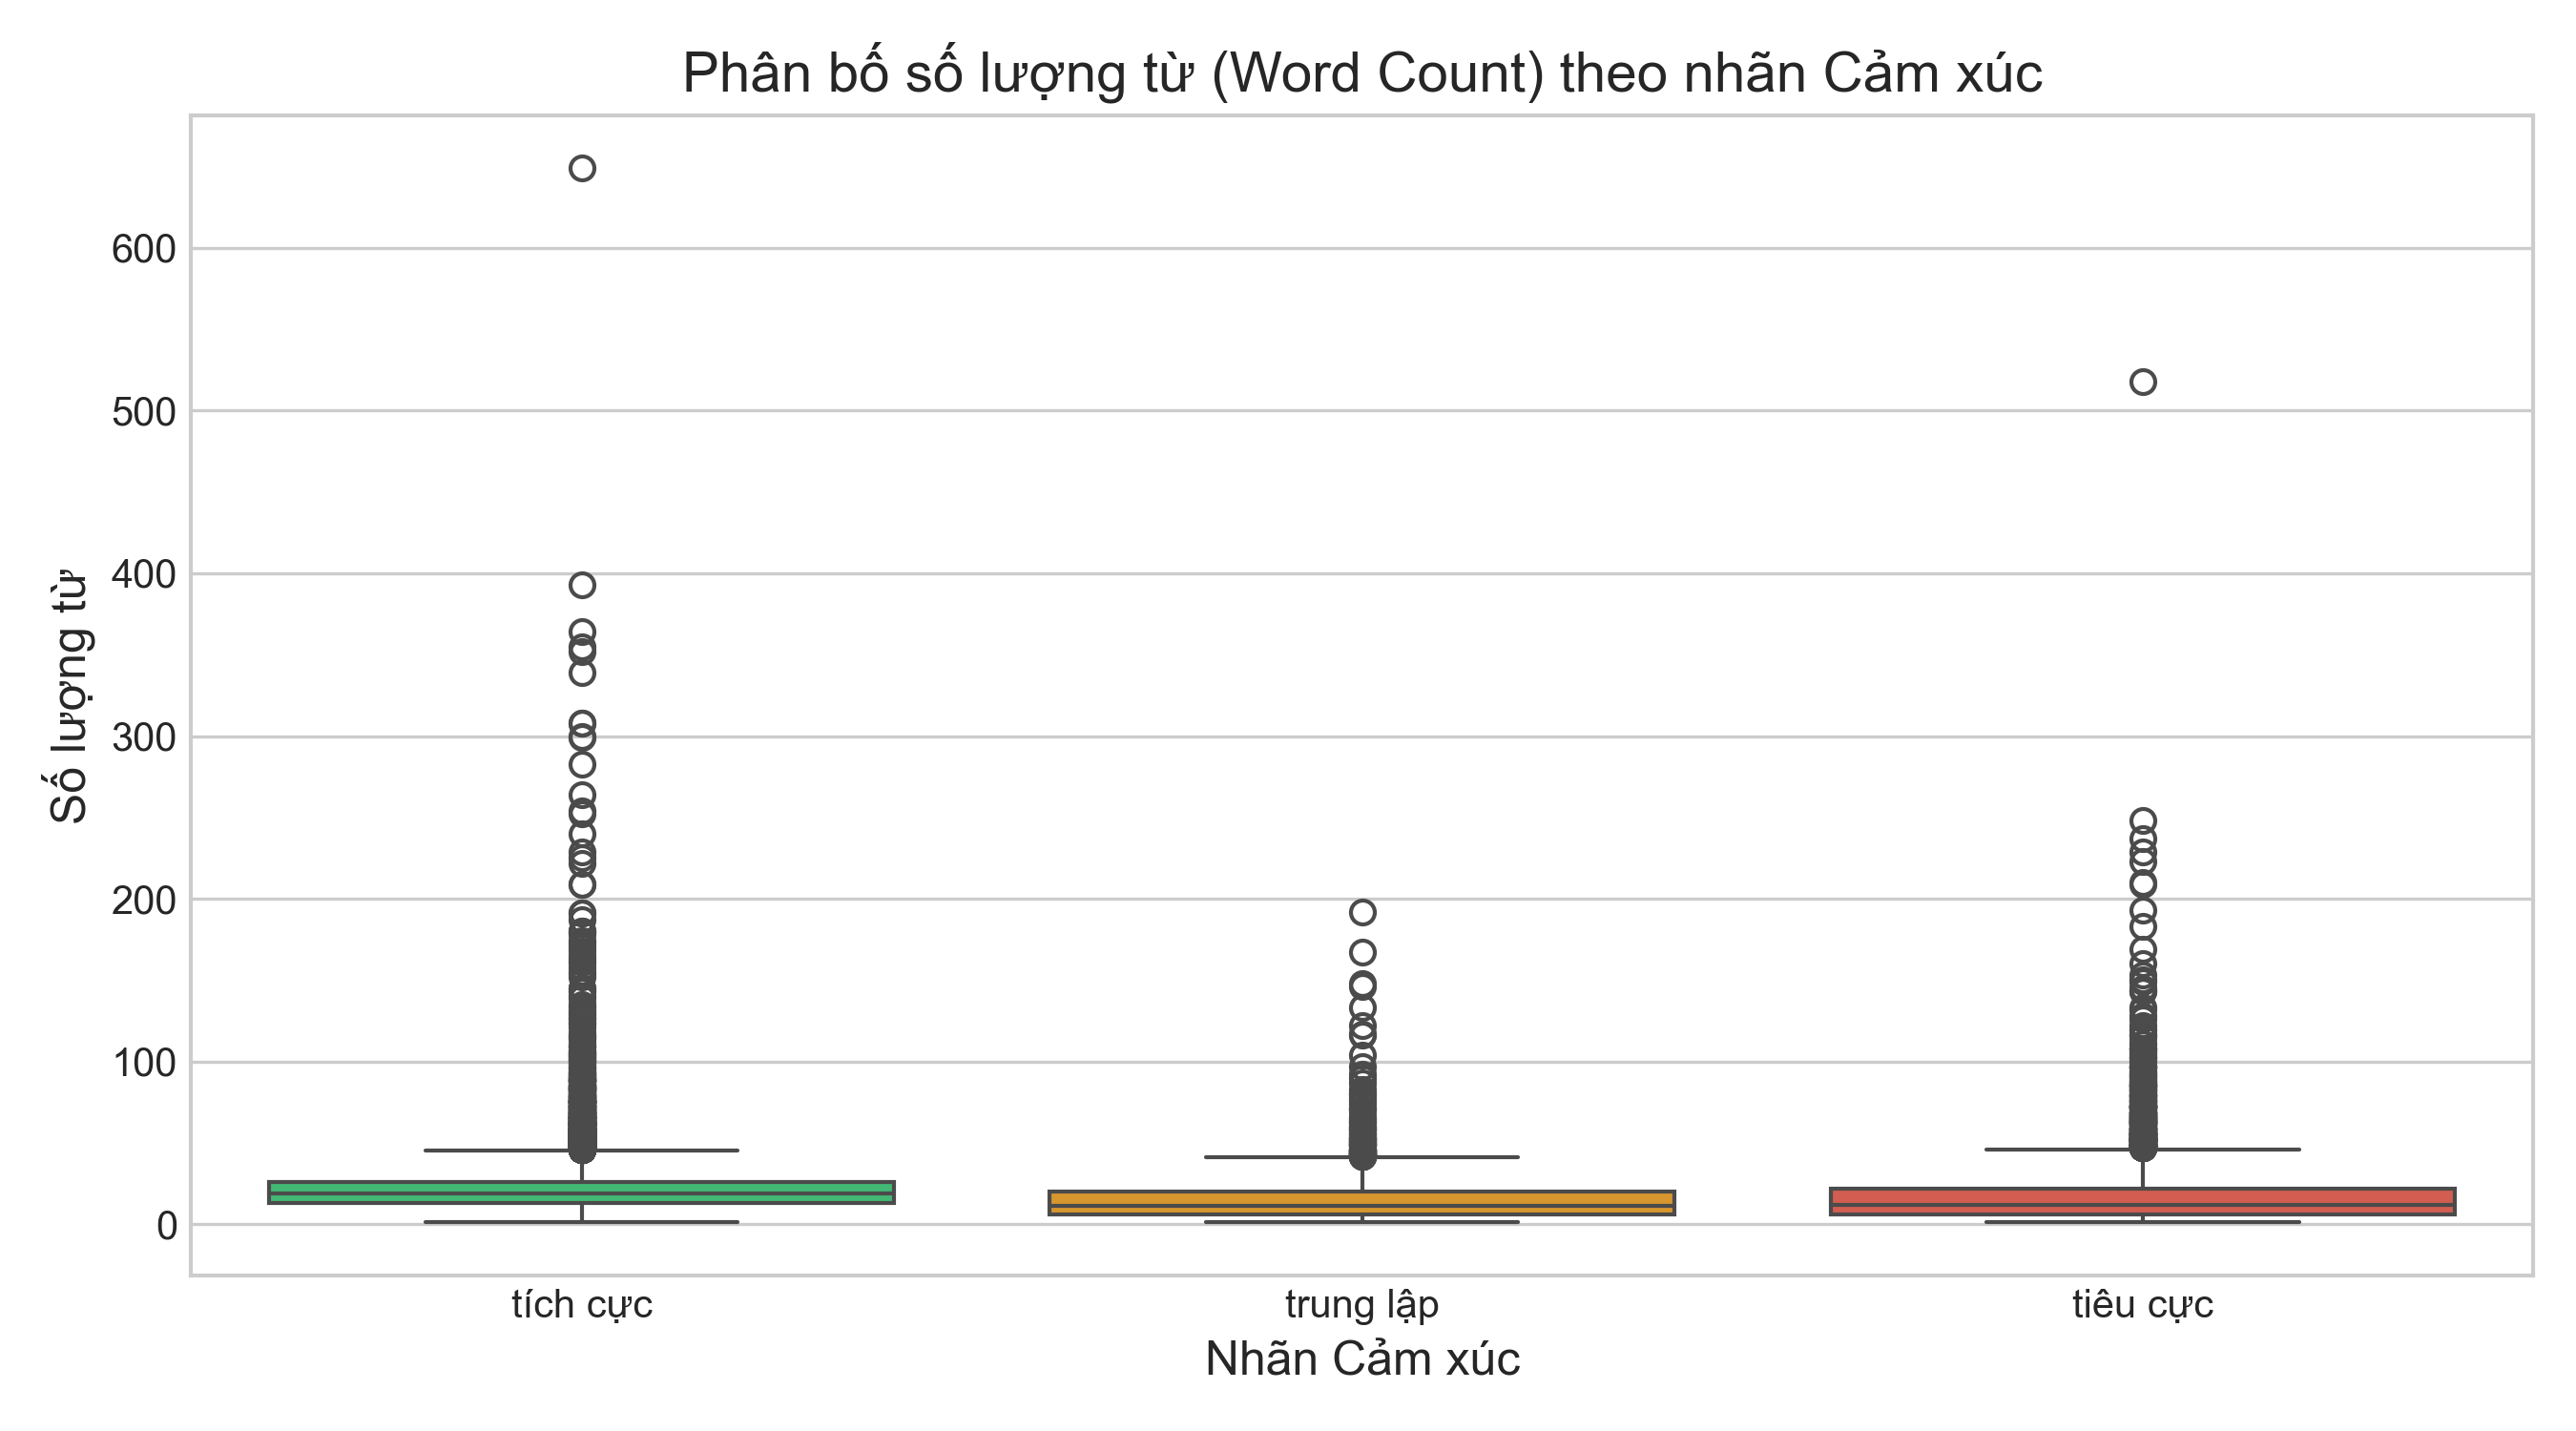
\includegraphics[width=0.85\textwidth]{graphics/text_word_count_boxplot.png}
    \caption[Phân bố độ dài văn bản]{%
      Phân bố độ dài văn bản.\\
      \textit{Ghi chú: Thống kê số lượng từ theo từng nhóm nhãn cảm xúc thông qua biểu đồ hộp.}%
    }
    \label{fig:text_word_count_boxplot}
\end{figure}

Biểu đồ hộp (Hình~\ref{fig:text_word_count_boxplot}) và các số liệu thống kê cho thấy \textit{nhóm bình luận tích cực có độ dài văn bản lớn nhất}. Điểm trung vị của nhóm tích cực đạt 19 từ, cao hơn so với nhóm tiêu cực (12 từ) và trung lập (11 từ). Đồng thời, phần đuôi phân phối (chứa các giá trị ngoại lai) của nhóm tích cực kéo dài tới tận 649 từ, vượt qua mức cực đại của nhóm tiêu cực (518 từ).

Đặc điểm này phản ánh thực trạng của các nền tảng thương mại điện tử: cơ chế tặng xu thưởng. Để nhận được lượng xu tối đa, người dùng buộc phải viết đánh giá dài kèm hình ảnh/video. Điều này dẫn đến việc khách hàng hài lòng có xu hướng viết dài, chèn thêm thơ ca, bài hát, hoặc sao chép các đoạn văn mẫu không liên quan để đạt đủ số lượng từ yêu cầu. Ngược lại, khi khách hàng gặp sự cố và đánh giá tiêu cực, họ thường tập trung đi thẳng vào vấn đề một cách súc tích (ví dụ: ``hàng rách'', ``giao sai mẫu'', ``quá tệ''), dẫn đến số lượng từ thấp hơn nhưng mật độ ngữ nghĩa lại cao. Đặc tính phân bố này cho thấy mô hình học máy cần tập trung khai thác các đặc trưng ngữ nghĩa sâu thay vì chỉ dựa vào độ dài bề mặt của văn bản.

\subsection{Phân tích đặc trưng và chiến lược xử lý dữ liệu hình ảnh}

Bên cạnh văn bản, hình ảnh đính kèm đóng vai trò quan trọng giúp xác thực nội dung đánh giá. Phần này tập trung khảo sát các nhãn hình ảnh đã thu thập và trình bày cách nhóm áp dụng kỹ thuật biến đổi ảnh tự động lúc huấn luyện.

\subsubsection{Phân bố các lớp ảnh khiếm khuyết}

Tập dữ liệu hình ảnh được gán nhãn thành 4 phân lớp độc lập nhằm hỗ trợ nhận diện tình trạng vật lý của kiện hàng hoặc sản phẩm: nguyên vẹn (\texttt{intact}), hư hỏng (\texttt{damaged}), giao sai hàng (\texttt{wrong\_item}), và không liên quan (\texttt{irrelevant}).

\begin{figure}[H]
    \centering
    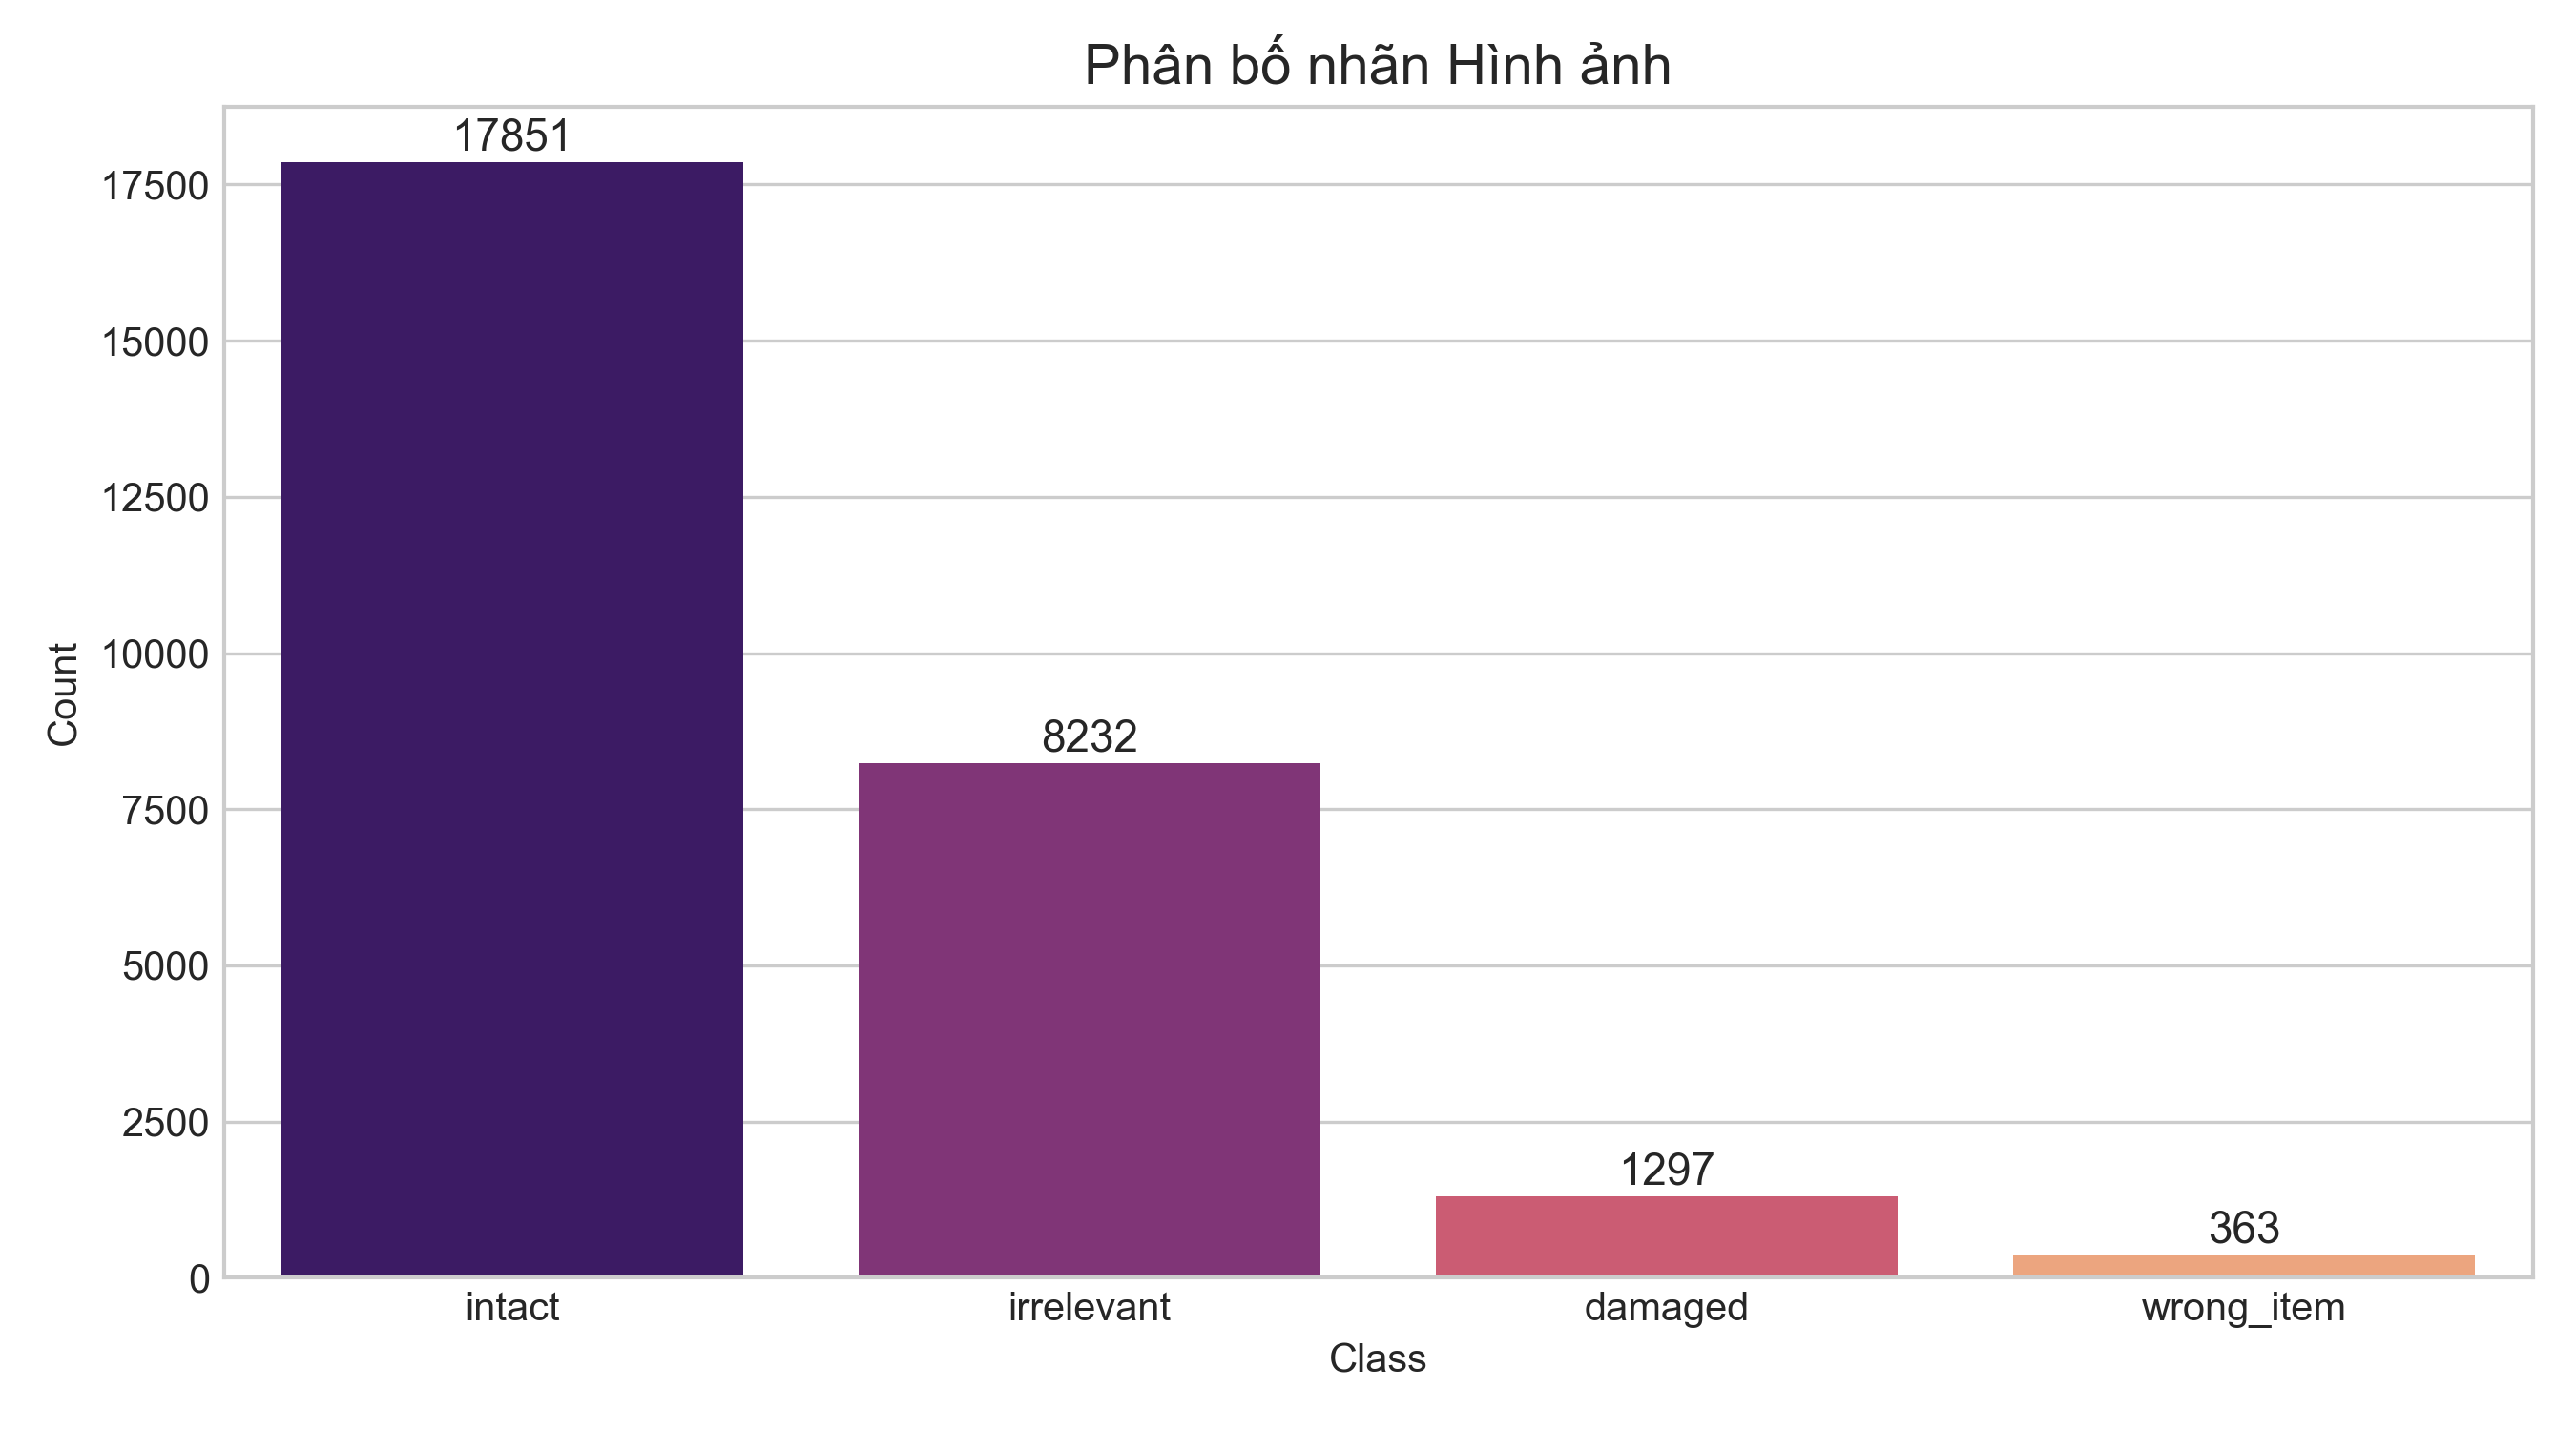
\includegraphics[width=0.85\textwidth]{graphics/image_distribution.png}
    \caption[Phân bố các lớp ảnh khiếm khuyết]{%
      Phân bố các lớp ảnh khiếm khuyết.\\
      \textit{Ghi chú: Thống kê số lượng hình ảnh được phân loại theo các tình trạng vật lý của sản phẩm.}%
    }
    \label{fig:image_distribution}
\end{figure}

Quan sát từ Hình~\ref{fig:image_distribution} cho thấy lớp ảnh nguyên vẹn (\texttt{intact}) sở hữu số lượng lớn nhất (17.851 mẫu), phản ánh đúng thực tế đa số các đơn hàng đều đến tay người dùng một cách bình thường. Đáng chú ý, đứng thứ hai là nhóm ảnh không liên quan (\texttt{irrelevant}) với 8.232 mẫu. Sự xuất hiện dày đặc của nhóm ảnh này xuất phát từ thói quen tải ảnh bất kỳ (ảnh thiên nhiên, thú cưng, ảnh mạng) để lách luật hệ thống nhằm nhận xu thưởng đánh giá trên các sàn giao dịch. Lớp hình ảnh hư hỏng (\texttt{damaged}) xếp thứ ba với 1.297 mẫu, và cuối cùng là giao sai hàng (\texttt{wrong\_item}) với 363 mẫu. Tỷ lệ lớn của nhóm \texttt{irrelevant} đặt ra bài toán thị giác máy tính quan trọng ở giai đoạn sau: mô hình cần hoạt động như một bộ lọc chéo (cross-modal filter). Nếu bình luận phàn nàn về chất lượng nhưng ảnh lại được dự đoán là \texttt{irrelevant}, hệ thống có thể kết luận mức độ tin cậy của đánh giá đó thấp.

\subsubsection{Chiến lược biến đổi hình ảnh động}

Trong luồng xử lý thị giác, thao tác tiền xử lý (đưa ảnh về cùng kích thước, chuẩn hóa cường độ điểm ảnh) và tăng cường dữ liệu là bắt buộc. Tuy nhiên, thay vì áp dụng biến đổi và lưu trữ toàn bộ tập ảnh mới ra bộ nhớ vật lý, hệ thống triển khai chiến lược biến đổi động ngay trong quá trình nạp dữ liệu. Quá trình này được thực thi thông qua thư viện \texttt{Albumentations} kết hợp cùng \texttt{DataLoader} của PyTorch.

Nhóm quyết định áp dụng cách làm này vì ba lý do chính:
\begin{itemize}[labelsep=10pt, leftmargin=2cm]
    \item \textbf{Tối ưu hóa tài nguyên vật lý và I/O:} Việc ngăn chặn sự bùng nổ dung lượng lưu trữ do không cần sao chép và ghi ra đĩa hàng chục nghìn biến thể của dữ liệu gốc giúp tiết kiệm không gian bộ nhớ. Đồng thời, việc đọc file một lần và áp dụng phép tính ma trận trong RAM bằng GPU sẽ giảm thiểu tắc nghẽn băng thông đọc/ghi ổ đĩa.
    \item \textbf{Chống hiện tượng overfitting:} Việc biến đổi động đảm bảo ở mỗi epoch, mô hình sẽ được tiếp xúc với một phiên bản tăng cường ngẫu nhiên khác nhau của cùng một bức ảnh gốc. Cụ thể, qua pipeline \texttt{get\_defect\_transforms()}, ảnh có thể bị xoay góc ngẫu nhiên, lật ngang, làm nhiễu sáng (Brightness/Contrast),... Tính ngẫu nhiên liên tục này làm tăng cường độ đa dạng của dữ liệu khổng lồ theo thời gian thực, ép buộc mô hình phải học các đặc trưng quang học bất biến của khiếm khuyết thay vì ghi nhớ cấu trúc nhiễu tĩnh.
    \item \textbf{Khả năng mở rộng và linh hoạt:} Pipeline cho phép tinh chỉnh, thêm bớt các phép biến đổi ngay lập tức trên mã nguồn mà không cần phải thực thi lại toàn bộ quy trình sinh file tiền xử lý mất hàng giờ đồng hồ.
\end{itemize}

\begin{figure}[H]
    \centering
    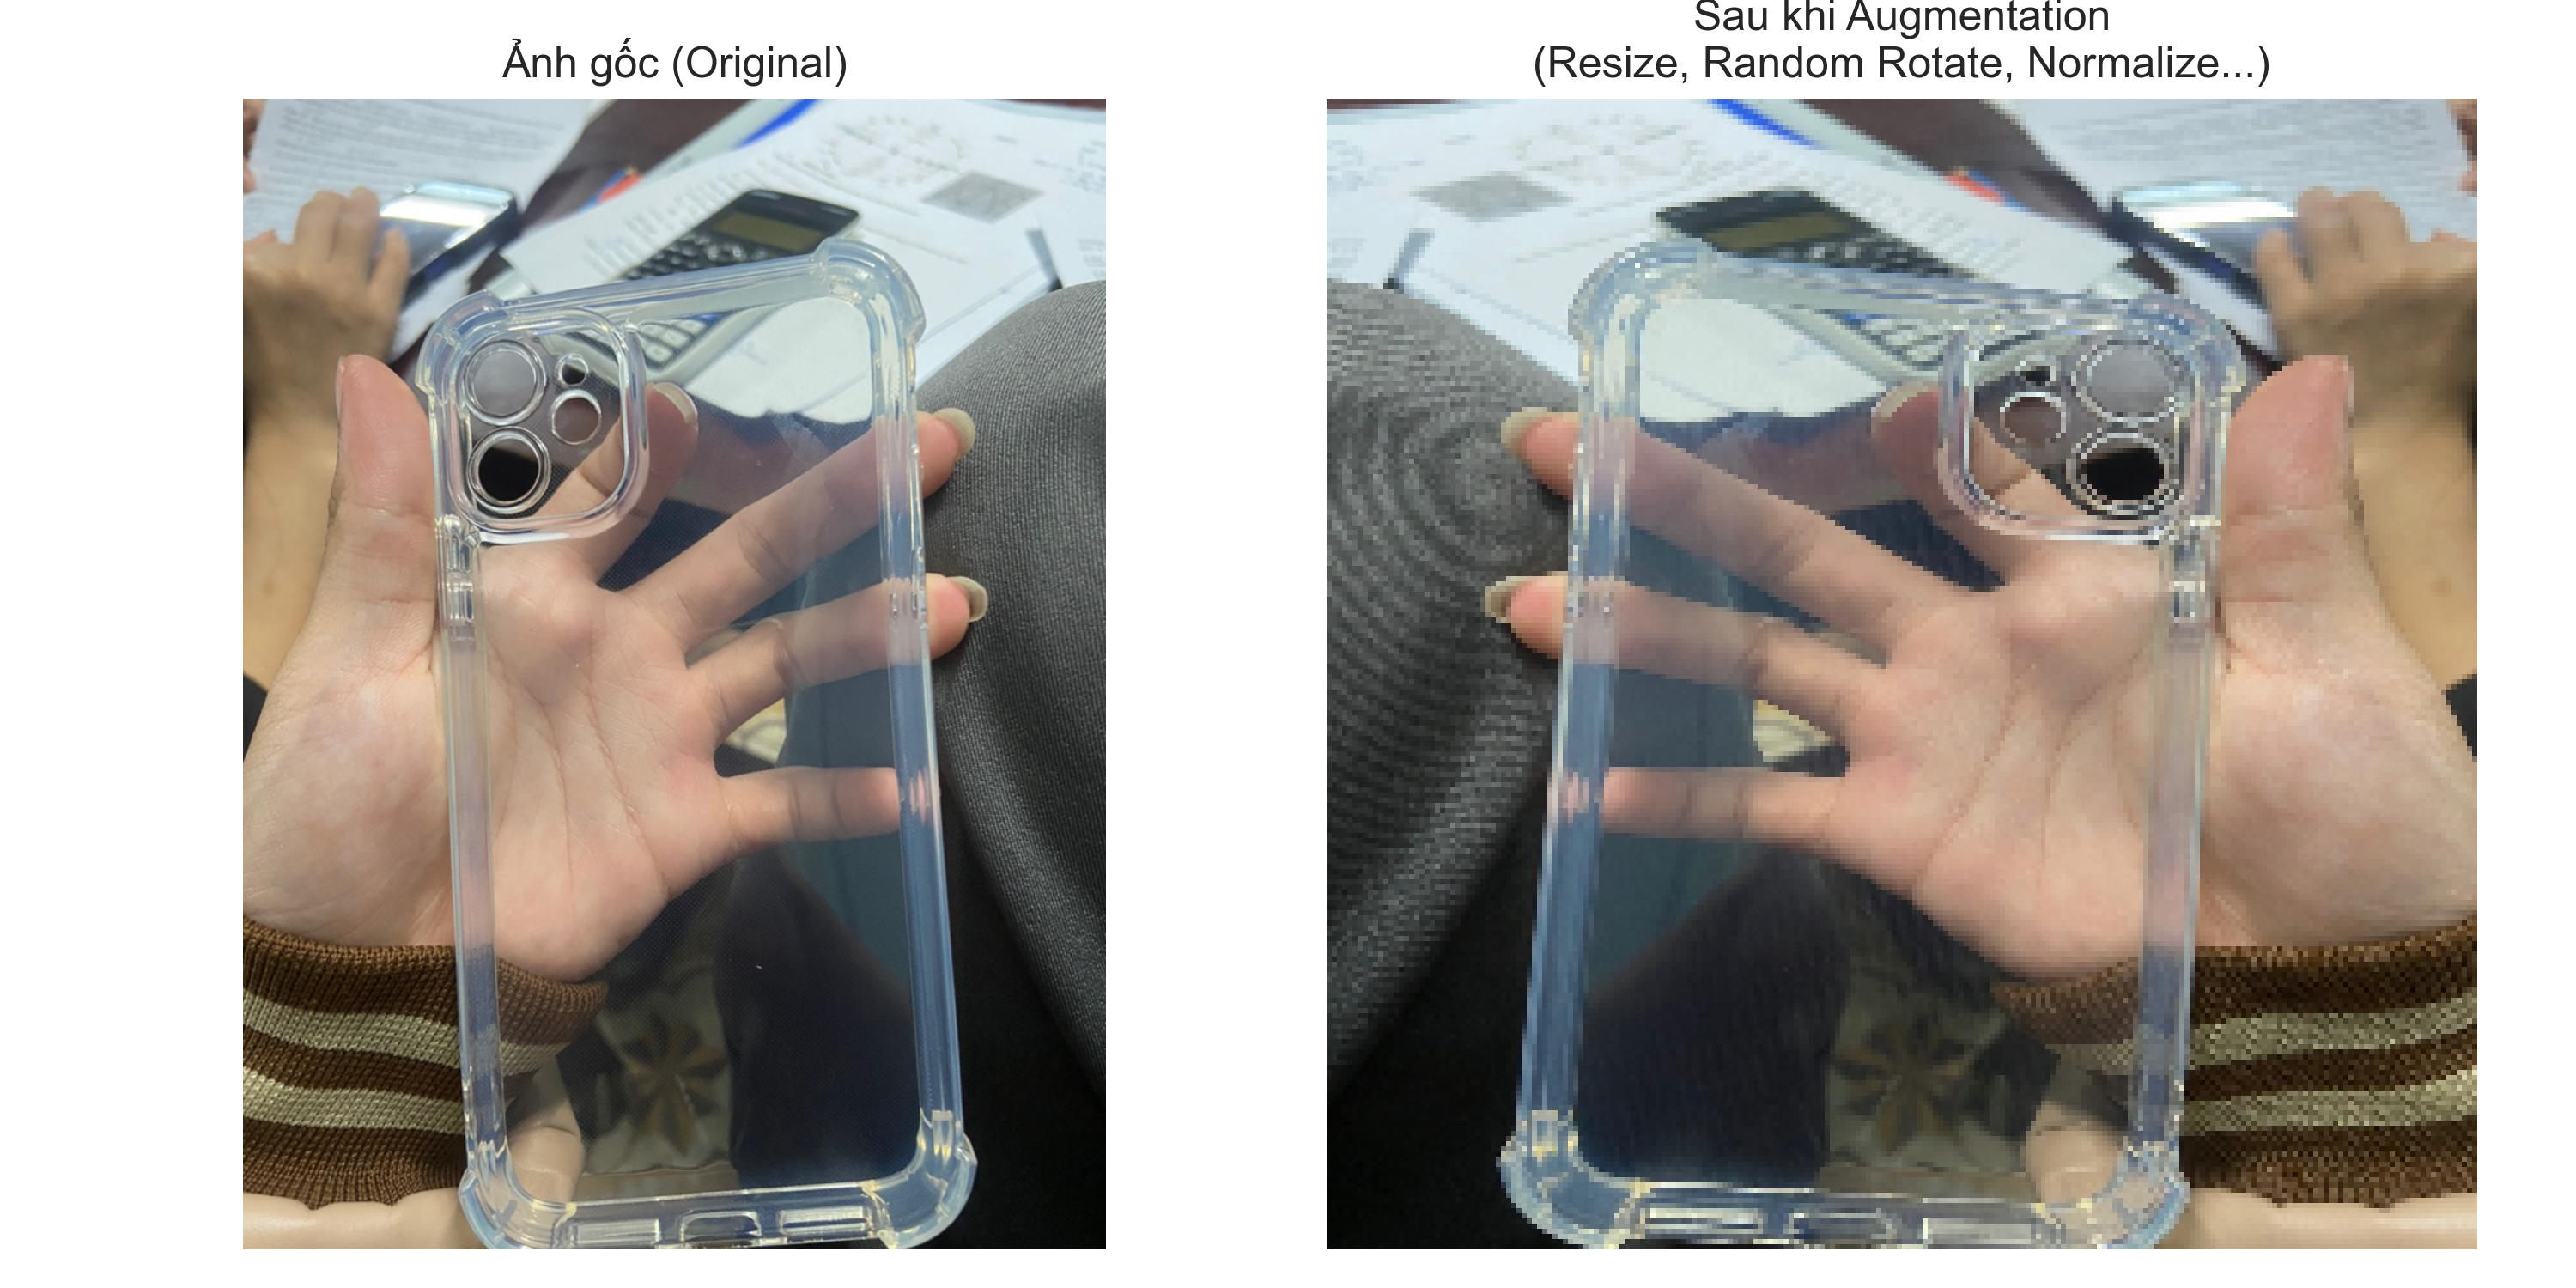
\includegraphics[width=\textwidth]{graphics/augmentation_demo.png}
    \caption[Minh họa biến đổi ảnh động (Augmentation)]{%
      Minh họa biến đổi ảnh động (Augmentation).\\
      \textit{Ghi chú: Ảnh bên trái là dữ liệu gốc, ảnh bên phải là kết quả ngẫu nhiên sau khi áp dụng thay đổi kích thước ($224 \times 224$), lật ngang và chuẩn hóa màu sắc thông qua đường ống \texttt{Albumentations}.}%
    }
    \label{fig:augmentation_demo}
\end{figure}

Hình~\ref{fig:augmentation_demo} thể hiện trực quan tác động của đường ống tăng cường dữ liệu lên một bức ảnh bị lỗi hư hỏng thực tế. Cường độ sáng và ma trận điểm ảnh đã được căn chỉnh (trừ đi mean và chia std) nhằm đạt mức phân phối tiêu chuẩn trước khi đưa vào các lớp học sâu của mạng nơ-ron thị giác. Sự khác biệt về hệ quy chiếu màu sắc giữa hai ảnh minh chứng rõ nét cho quá trình Normalize.

\subsection{Phân chia tập huấn luyện và kiểm thử}

Quá trình phân chia tập dữ liệu đóng vai trò quyết định trong việc đánh giá khách quan khả năng tổng quát hóa của mô hình học máy trên dữ liệu thực tế chưa từng gặp. Dựa trên quy mô tổng cộng 25.292 bản ghi văn bản, nhóm nghiên cứu thiết lập tỷ lệ phân chia 70:15:15, tương ứng với ba tập: Huấn luyện (Train), Kiểm định (Validation) và Kiểm thử (Test).

\begin{itemize}[labelsep=10pt, leftmargin=2cm]
    \item \textbf{Tập Huấn luyện (70\% - 17.704 mẫu):} Được sử dụng trực tiếp để cập nhật trọng số và tối ưu hóa hàm mất mát của mạng nơ-ron hoặc các thuật toán học máy cơ sở.
    \item \textbf{Tập Kiểm định (15\% - 3.794 mẫu):} Hoạt động như một bộ lọc trung gian, hỗ trợ theo dõi hiệu suất mô hình qua từng vòng lặp (epoch). Từ đó, nhóm tiến hành tinh chỉnh các siêu tham số (hyperparameters) và áp dụng cơ chế dừng sớm (Early Stopping) nhằm ngăn chặn hiện tượng overfitting.
    \item \textbf{Tập Kiểm thử (15\% - 3.794 mẫu):} Bị cô lập hoàn toàn trong suốt quá trình phát triển mô hình. Tập dữ liệu này chỉ được sử dụng ở bước cuối cùng để đo lường độ chính xác và xuất ra các ma trận nhầm lẫn (Confusion Matrix) khách quan nhất.
\end{itemize}

Đặc biệt, do tính chất mất cân bằng cực đoan của nhãn cảm xúc (lớp tích cực chiếm tới 64,6\% trong khi lớp trung lập chỉ đạt 7,7\%), phương pháp trích mẫu ngẫu nhiên thông thường (Random Sampling) có nguy cơ tạo ra các tập Kiểm định hoặc Kiểm thử thiếu vắng hoàn toàn lớp thiểu số. Do đó, nhóm nghiên cứu đã áp dụng kỹ thuật \textbf{Trích mẫu phân tầng (Stratified Split)} trong suốt quá trình chia tách. Kỹ thuật này đảm bảo tỷ lệ phân bố của cả ba nhãn cảm xúc và nhãn bình luận rác được giữ nguyên một cách đồng nhất trên toàn bộ ba tập dữ liệu. Điều này thiết lập một thước đo công bằng, buộc mô hình phải học cách phân biệt các lớp dữ liệu hiếm thay vì chỉ phỏng đoán theo xác suất của lớp đa số.

\vspace{0.5em}
\noindent\textbf{Đối với nhánh hình ảnh:}\\
Quá trình phân chia cũng tuân thủ nguyên tắc tương tự để phục vụ việc trích xuất đặc trưng hình ảnh. Tập dữ liệu ảnh gồm tổng cộng 27.743 mẫu được phân chia theo tỷ lệ \textbf{80:20} (tương ứng với 80\% Huấn luyện và 20\% Kiểm định) ngay trong bộ nạp dữ liệu (\texttt{get\_defect\_dataloaders}). Việc không tạo tập Test thứ ba độc lập giúp tiết kiệm không gian và gia tăng tối đa lượng ảnh cho pha Huấn luyện, do mô hình xử lý ảnh yêu cầu tài nguyên dữ liệu lớn hơn nhiều so với văn bản. 

Đồng thời, hàm chia tách vẫn giữ tham số \texttt{stratify} dựa trên 4 nhãn của ảnh (\texttt{intact}, \texttt{irrelevant}, \texttt{damaged}, \texttt{wrong\_item}). Điều này vô cùng quan trọng vì nhãn \texttt{wrong\_item} chỉ chiếm vỏn vẹn hơn 1\% tổng số dữ liệu (363 mẫu), nếu chia ngẫu nhiên, tập Validation có thể không chứa bức ảnh giao sai hàng nào, dẫn đến sai lệch nghiêm trọng khi đánh giá chất lượng hội tụ của bộ trích xuất đặc trưng thị giác.